\documentclass[../../main]{subfiles}

\renewcommand\thesection{\arabic{section}}


\begin{document}

\section{GUI App} \label{sec:}

\begin{figure}
    \centering

    {\hfill
    \begin{minipage} {0.3\textwidth}
        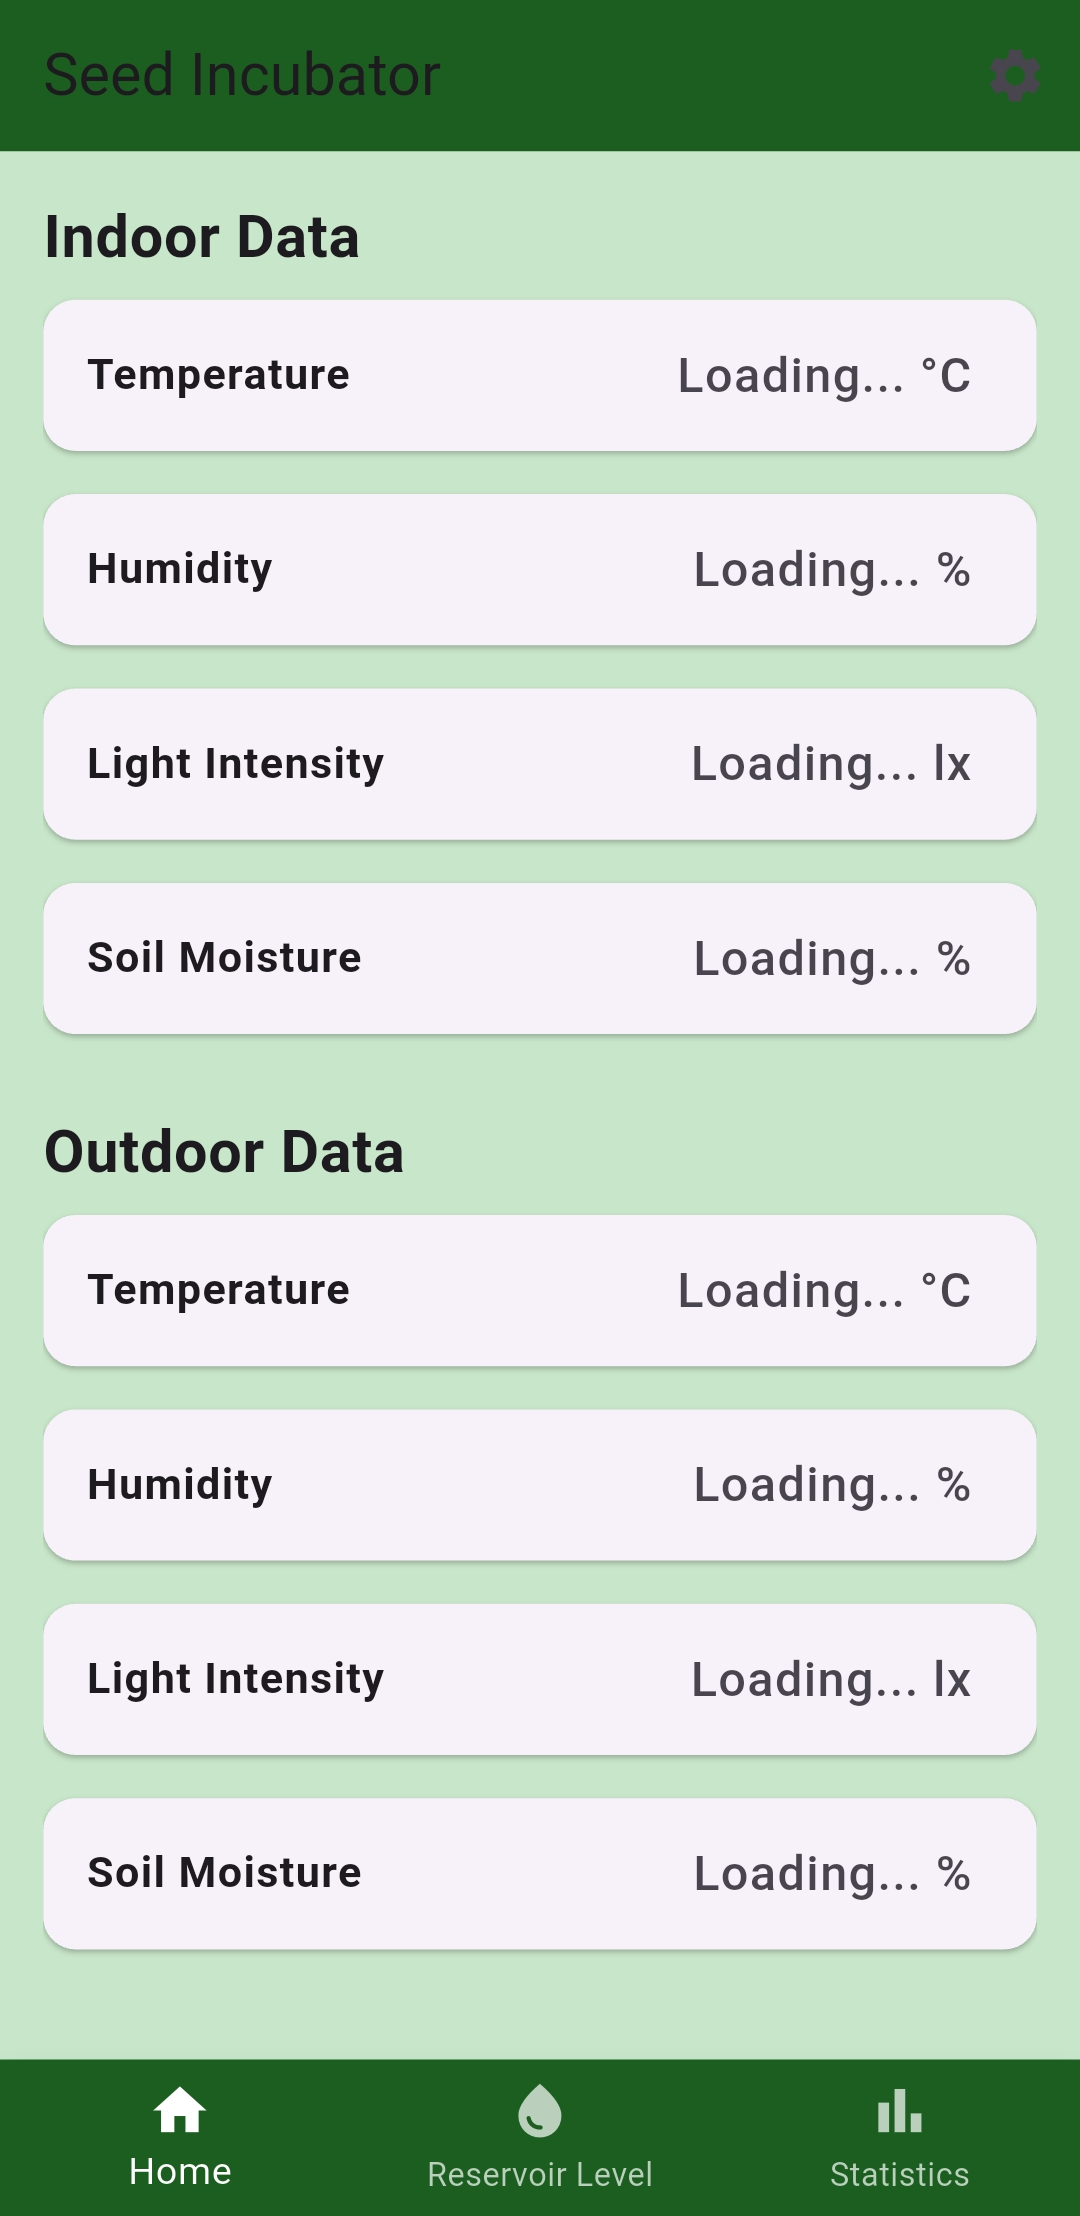
\includegraphics [
            max width = \IGXMaxWidth,
            max height = \IGXMaxHeight,
            \IGXDefaultOptionalArgs,
        ] {pics/s1.jpg}

    \end{minipage}
    \hfill
    \begin{minipage} {0.3\textwidth}
        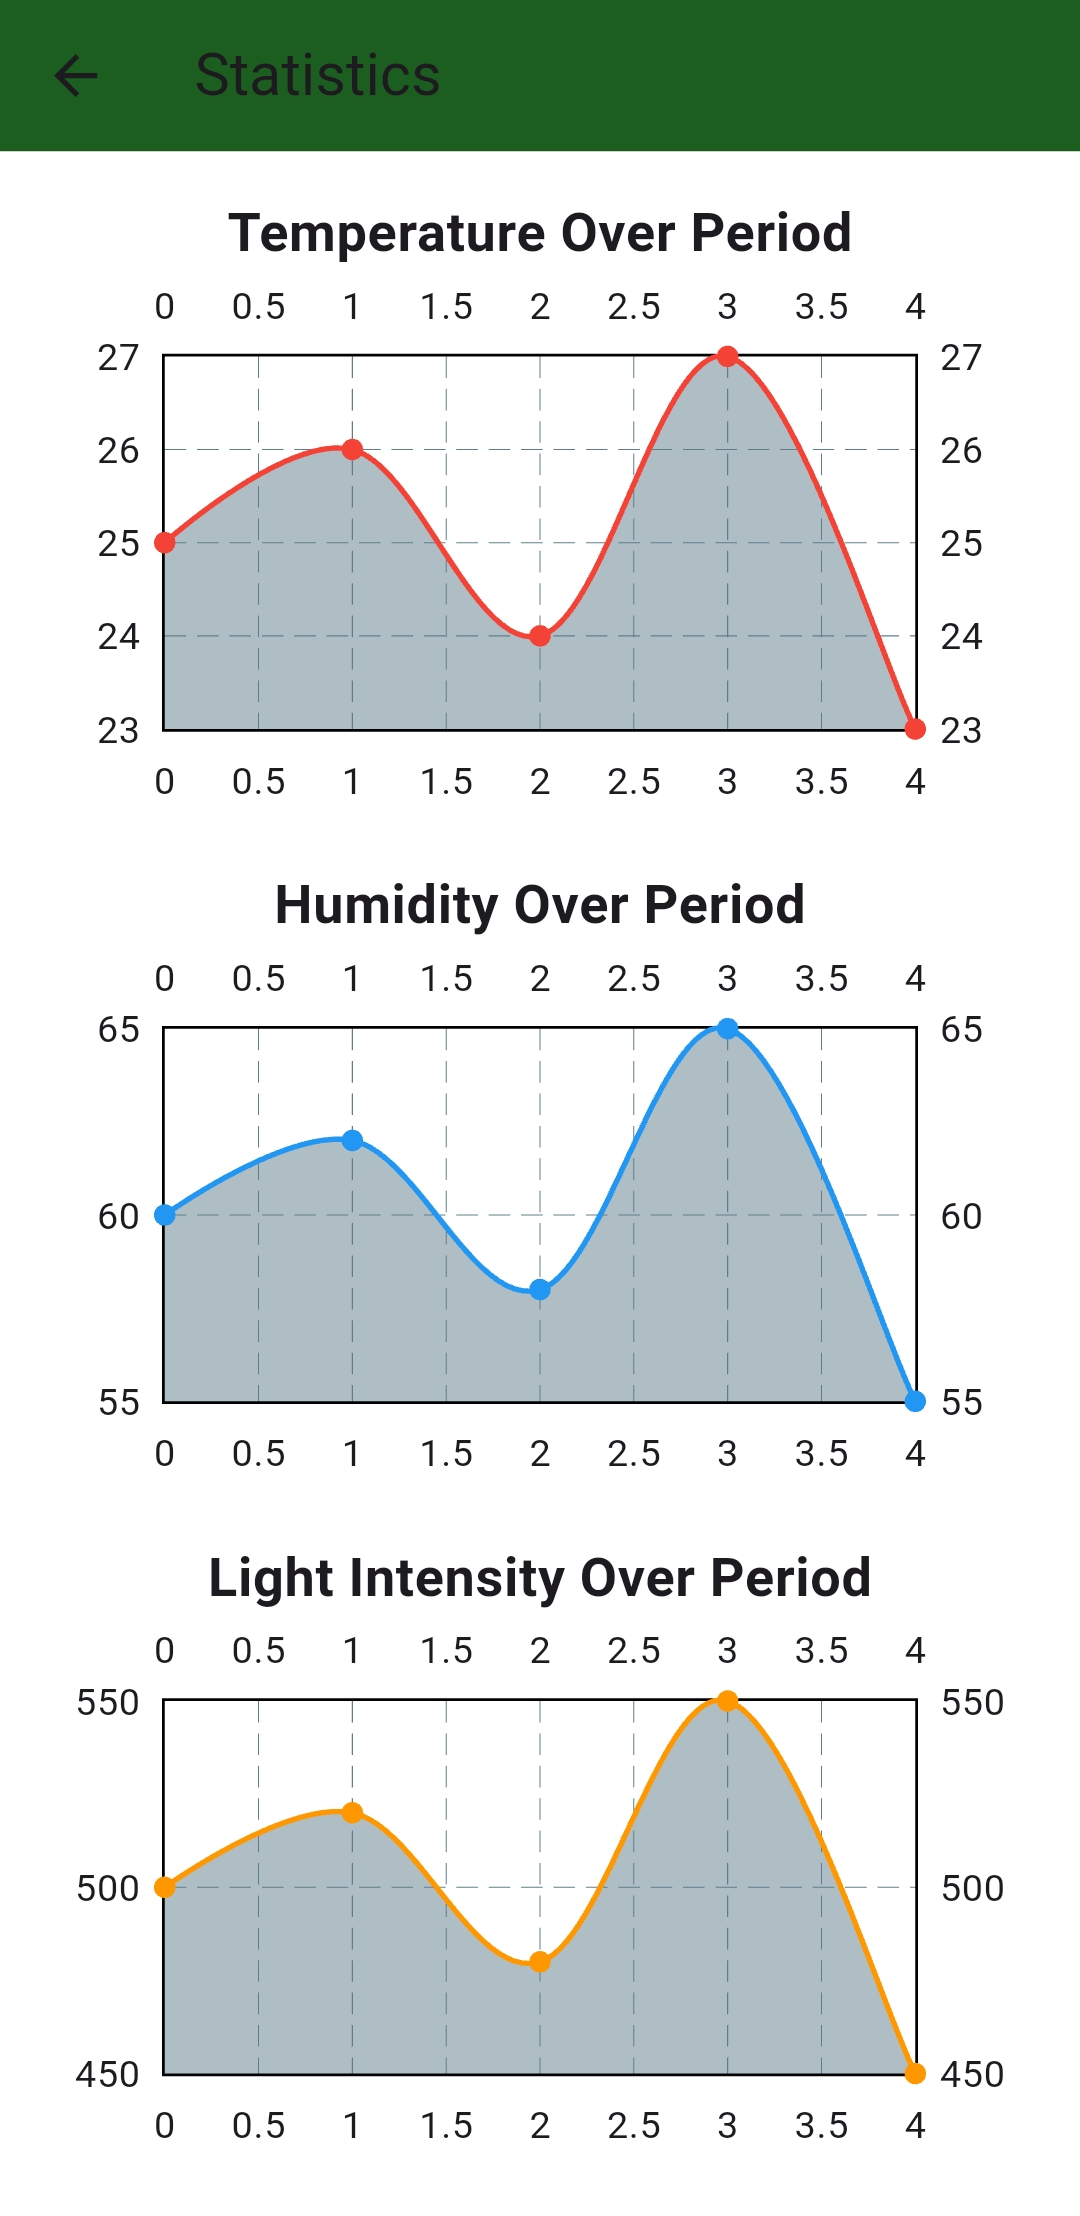
\includegraphics [
            max width = \IGXMaxWidth,
            max height = \IGXMaxHeight,
            \IGXDefaultOptionalArgs,
        ] {pics/s2.jpg}

    \end{minipage}
    \hfill
    \begin{minipage} {0.3\textwidth}
        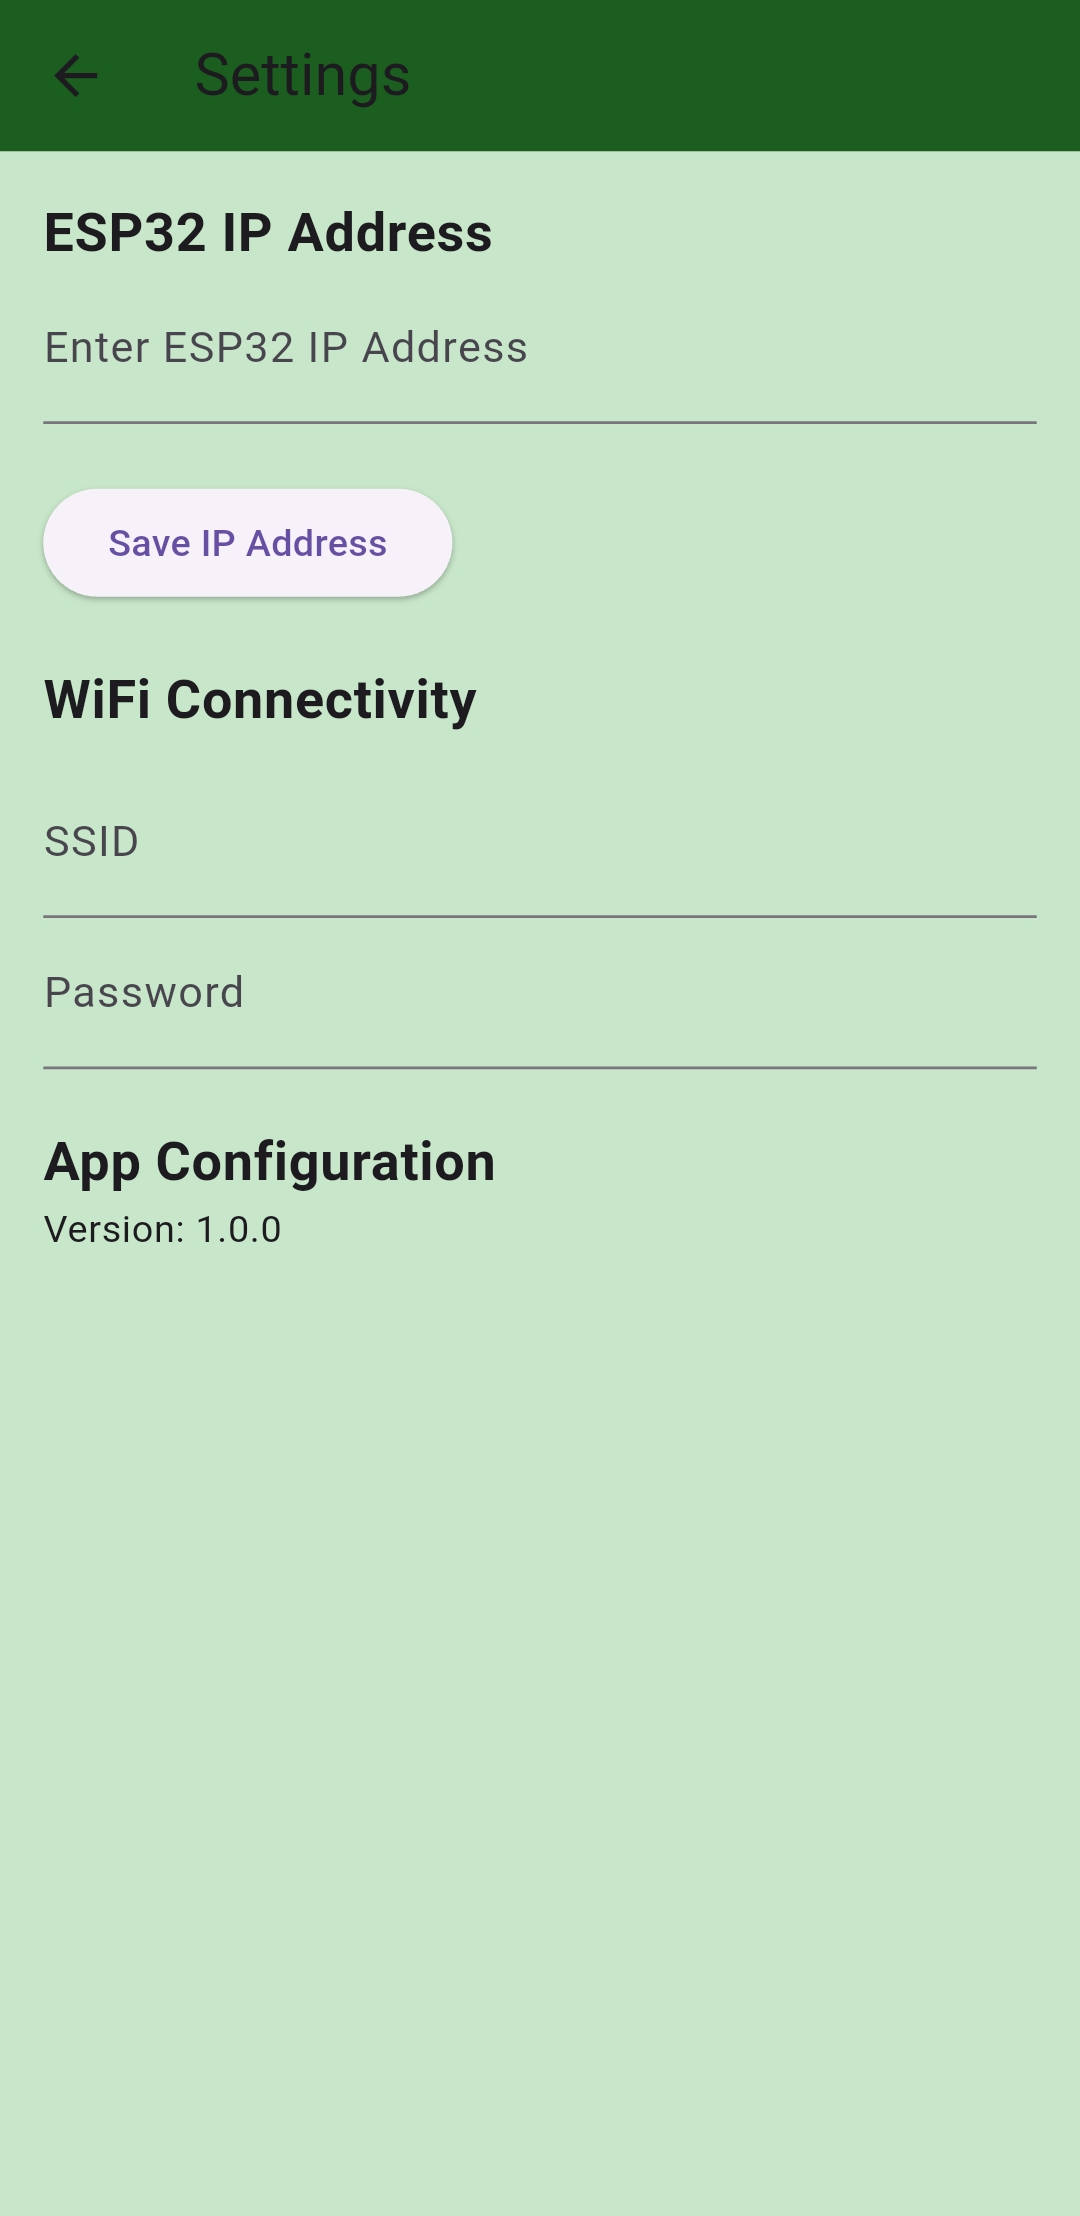
\includegraphics [
            max width = \IGXMaxWidth,
            max height = \IGXMaxHeight,
            \IGXDefaultOptionalArgs,
        ] {pics/s3.jpg}

    \end{minipage}
    \hfill}

    \captionof{figure} {Screenshots of GUI SINC App.}
    \label{fig:}

\end{figure}

\alertNote{
    Right now, the only the UI of the GUI app is done. Backend is not implemented yet.
}

\end{document}
